% \begin{figure*}[ht!]
% \centering
% 	\begin{subfigure}{0.48\textwidth}
%                 \centering
% 		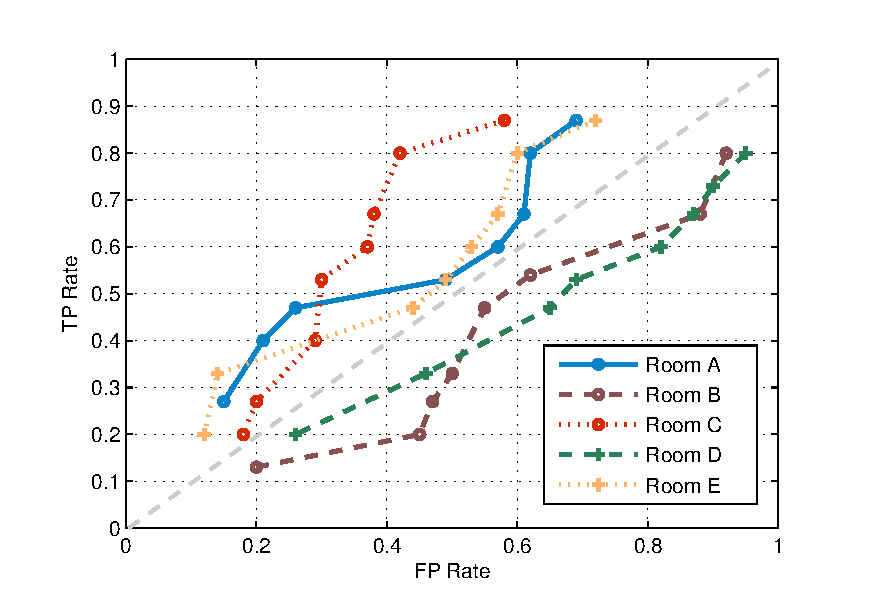
\includegraphics[width=\textwidth]{./fig/ROC_bsln.eps}
%                 \caption{Correlating the raw signals.}
% 	\end{subfigure}
% 	\begin{subfigure}{0.48\textwidth}
%                 \centering
% 		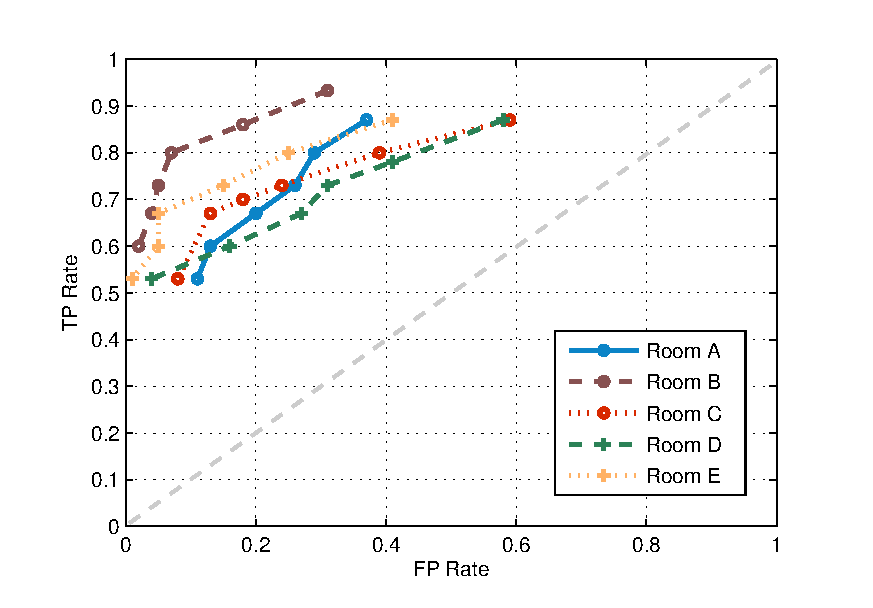
\includegraphics[width=\textwidth]{./fig/ROC_new.eps}
%                 \caption{Correlating the re-aggregated IMFs in the ``medium'' frequency band.}
%                 \label{fig:rocA}
% 	\end{subfigure}
% \caption{The ROC curves depict the sensitivity of the raw signal and mid-frequency IMFs to the threshold value. We choose the 0.2 FPR point as the boundary threshold for each room. }
% \label{fig:roc}
% \end{figure*}

\section{Evaluation}
To demonstrate the effectiveness as well as usefulness of our methodology, we evaluate our technique in two different scenarios: a) intra building, that is, the 
training and testing data for classification is taken from the same building, and b) inter buildings, where the training and testing instances are from two 
distinct buildings. Then we analyze how the window size of segment and number of training instances affect the performance of classification. We also discuss how 
each feature variable contributes to the classification and when to use certain set of features. At last, we show a small application as a case study built based on 
the generated type information in two buildings, which would be difficult to achieve in the absence of sensor type metadata. 

\subsection{Taxonamy}
In this paper, we consider 6 types of sensors, which are $CO_{2}$, humidity, room temperature, setpoint, air flow volume, other temperature. Specifically, room 
temperature includes only sensors that measure the air temperature of rooms and other temperatures covers all other temperature measurements such as supply 
air/return air/mixed air temperature and supply/return water temperature. We also put only one general type for setpoint which includes all types of setpoints 
installed in the buildings.

\subsection{Experimental Setup}
The data we used are collected in one week from two separate buildings on two campuses. One is from the Sutardja Dai Hall at UC Berkeley where the deployed 
sensors~\cite{keti, bacnet} report to an archiver~\cite{smap} periodically from every 5 seconds to every 10 minutes. The other building is the Rice Hall at 
University of Virginia, where the sensors report to a central database~\cite{trane} from every 10 seconds to every 10 minutes. The number of each type of sensors in 
each buidlings is given in table~\ref{table:spec}.

\begin{table}[ht!]
\caption{Number of Each Sensor Type}
\centering % used for centering table
\begin{tabular}{c c c}% centered columns (4 columns)
\hline %inserts single horizontal lines
Type & SDH & Rice \\ % inserts table 
%heading
\hline\hline % inserts double horizontal line
$CO_{2}$ & 1 & 2 \\ % inserting body of the table
humidity & 2 & 4 \\
room temp. & 3 & 2 \\
setpoint & 4 & 7 \\
air volume & 5 & 5 \\ % [1ex] adds vertical space
other temp. & 6 & 5 \\ % [1ex] adds vertical space
\hline %inserts single line
\end{tabular}
\label{table:spec} % is used to refer this table in the text
\end{table}

\subsection{Baseline and Metrics}
As a baseline to compare our proposed approach against, we adpot a simple feature extraction scheme for each trace $F=\{med, var\}$, where $med$ and $var$ is just the $median$ and $variance$ computed over the entire trace.

For classification, we measure the averaged cross-validation accuracy in two different scenarios (intra- and inter- buildings). For identifying potential 
misclassifications, we choose the true-positive rate (TPR, also known as recall rate) and false-positive rate (FPR) as metrics to evaluate the performance of 
our entropy-based aprroach. In our case, a true-positive (TP) is when an instance considered to be misclassified is actually a correct classification while a 
false-positive (FP) is when an instance considered to be misclassfied is misclassified.

\subsection{Intra Building Performance}
\begin{table}[ht!]
\caption{Type Classification Accuracy for SDH}
\centering % used for centering table
\begin{tabular}{c | c | c | c | c | c | c}% centered columns (4 columns)
\hline %inserts single horizontal lines
Type & 5\% & 10\% & 20\% & 33\% & 50\% & LOO \\ % inserts table 
%heading
\hline\hline % inserts double horizontal line
$CO_{2}$ & 1 & 2 & 1 & 2 & 1 & 1 \\ % inserting body of the table
\hline %inserts single line
Humidity & 2 & 4 & 1 & 2 & 1 & 1 \\
\hline %inserts single line
Room temp. & 3 & 2 & 1 & 2 & 1 & 1 \\
\hline %inserts single line
Setpoint & 4 & 7 & 1 & 2 & 1 & 1 \\
\hline %inserts single line
Air volume & 5 & 5 & 1 & 2 & 1 & 1 \\ % [1ex] adds vertical space
\hline %inserts single line
Other temp. & 6 & 5 & 1 & 2 & 1 & 1 \\ % [1ex] adds vertical space
\hline %inserts single line
Overall & 6 & 5 & 1 & 2 & 1 & 1 \\ % [1ex] adds vertical space
\hline %inserts single line
\end{tabular}
\label{table:sdh} % is used to refer this table in the text
\end{table}

\begin{table}[ht!]
\caption{Type Classification Accuracy for Rice Hall}
\centering % used for centering table
\begin{tabular}{c | c | c | c | c | c | c}% centered columns (4 columns)
\hline %inserts single horizontal lines
Type & 5\% & 10\% & 20\% & 33\% & 50\% & LOO \\ % inserts table 
%heading
\hline\hline % inserts double horizontal line
$CO_{2}$ & 1 & 2 & 1 & 2 & 1 & 1 \\ % inserting body of the table
\hline %inserts single line
Humidity & 2 & 4 & 1 & 2 & 1 & 1 \\
\hline %inserts single line
Room temp. & 3 & 2 & 1 & 2 & 1 & 1 \\
\hline %inserts single line
Setpoint & 4 & 7 & 1 & 2 & 1 & 1 \\
\hline %inserts single line
Air volume & 5 & 5 & 1 & 2 & 1 & 1 \\ % [1ex] adds vertical space
\hline %inserts single line
Other temp. & 6 & 5 & 1 & 2 & 1 & 1 \\ % [1ex] adds vertical space
\hline %inserts single line
Overall & 6 & 5 & 1 & 2 & 1 & 1 \\ % [1ex] adds vertical space
\hline %inserts single line
\end{tabular}
\label{table:rice} % is used to refer this table in the text
\end{table}

\subsection{Inter Building Performance}

\begin{table*}[ht!]
\caption{Type Classification Accuracy for SDH}
\centering % used for centering table
\begin{tabular}{c | c | c | c | c | c}% centered columns (4 columns)
\hline %inserts single horizontal lines
Type & 5\% & 10\% & 20\% & 33\% & 50\% \\ % inserts table 
%heading
\hline\hline % inserts double horizontal line
$CO_{2}$ & 63.5 (39.5) & 96.9 (4.7) & 90.8 (16.5) & 93.6 (4.8)  & 92.3 (1.9)\\ \hline
Humidity & 67.4 (35.4) & 86.3 (27.8) & 98.1 (2.1) & 96.2 (2.7)  & 98.1 (1.9)\\ \hline
Room temp & 78.0 (18.5) & 78.2 (11.3) & 72.9 (3.3) & 77.9 (3.4)  & 80.3 (3.5)\\ \hline
Setpoint & 77.4 (17.1) & 83.3 (8.6) & 86.5 (8.7) & 87.9 (5.5) & 87.2 (3.5)\\ \hline
Air volume & 13.8 (18.7) & 15.2 (11.8) & 37.8 (11.1) & 42.4 (12.3) & 50.3 (2.7)\\ \hline
Other temp & 48.3 (10.3) & 49.7 (5.4) & 58.4 (9.0) & 45.0 (6.4) & 45.9 (5.4)\\ \hline
Overall & 68.2 (10.9) & 74.1 (5.3) & 78.4 (5.0) & 80.3 (2.1) & 81.2 (5.9)\\ \hline
\end{tabular}
\label{table:sdh_x} % is used to refer this table in the text
\end{table*}

\begin{table*}[ht!]
\caption{Type Classification Accuracy for Rice Hall}
\centering % used for centering table
\begin{tabular}{c | c | c | c | c | c}% centered columns (4 columns)
\hline %inserts single horizontal lines
Type & 5\% & 10\% & 20\% & 33\% & 50\% \\ % inserts table 
%heading
\hline\hline % inserts double horizontal line
$CO_{2}$ & 29.7 (17.9) & 45.6 (22.7) & 75.0 (16.3) & 93.8 (5.1)  & 93.8 (6.3)\\ \hline
Humidity & 50.9 (18.8) & 72.1 (14.5) & 76.2 (9.6) & 76.4 (6.4)  & 89.6 (2.1)\\ \hline
Room temp & 97.6 (6.7) & 99.4 (1.5) & 100.0 (0) & 97.2 (3.5)  & 100.0 (0)\\ \hline
Setpoint & 97.8 (1.8) & 98.2 (1.4) & 98.0 (1.2) & 97.7 (0.3) & 97.5 (0.5)\\ \hline
Air volume & 57.5 (16.8) & 58.3 (17.5) & 66.7 (7.5) & 63.9 (10.4) & 70.8 (12.5)\\ \hline
Other temp & 5.3 (4.9) & 10.8 (6.2) & 11.1 (4.3) & 16.8 (4.1) & 18.9 (5.5)\\ \hline
Overall & 73.1 (2.1) & 76.9 (2.3) & 78.3 (2.0) & 79.1 (0.2) & 81.3 (0.7)\\ \hline
\end{tabular}
\label{table:rice_x} % is used to refer this table in the text
\end{table*}

\subsection{Window Length Sensitivity and Training Bootstrapping}

\subsection{Feature Importance and Selection}

\subsection{Identifying Misclassification}

\subsection{Case Study}
